
\begin{frame}{Splitting functions}
  Complete results for the N3LO splitting functions are not yet available, but a lot of information exists (with important contributions from Liverpool and Edinburgh):
  \begin{itemize}
    \item Small-x limits (BFKL resummation) {\color{gray}\footnotesize [Bonvini and Marzani: 1805.06460] [Davies, Kom, Moch, Vogt, 2202.10362]}
    \item Large-x limits (threshold resummation) {\color{gray}\footnotesize [Soar, Moch, Vermaseren, Vogt: 0912.0369], [Henn, Korchemsky, Mistlberger, 1911.10174], [Duhr, Mistlberger, Vita 2205.04493]}
    \item Large-$n_f$ limit {\color{gray}\footnotesize [Davies, Ruijl, Ueda, Vermaseren, Vogt: 1610.0744], [Gehrmann, Manteuffel, Sotnikov, Yan, 2308.07958]}
    \item Mellin moments
    {\color{gray}\footnotesize [Falcioni, Herzog, Moch, Ruijl, Ueda, Vermaseren, Vogt, 1707.08315, 2111.15561, 2302.07593, 2307.04158]}
  \end{itemize}

  \vspace*{2em}
  \begin{center}
    How can we use this information to construct approximate splitting functions?
  \end{center}

\end{frame}


\begin{frame}{DIS variable flavor number scheme (VFNS)}
  \begin{columns}
    \begin{column}{0.59\textwidth}
      \begin{itemize}
        \item In a PDF fit different flavour number schemes are joined in a variable flavour number scheme (VFNS) to ensure reliable results from $Q^2\sim m_h^2$ up to $Q^2\gg m_h^2$
        \item The matching conditions encoding the transition between schemes have almost completely been computed up to N3LO
        \item The VFNS used in NNPDF is the FONLL scheme
        % \item FONLL extended for arbitrary number of mass scales in the recent \texttt{EKO} (DGLAP) and \texttt{yadism} (DIS) codes
      \end{itemize}

      \vspace*{1em}
      \begin{equation*}
        F_\mathrm{FONLL}(m_c) =F^{(n_f+1)}(m_h=0)
        +F^{(n_f)}(m_c)-\lim_{m_c\rightarrow 0}F^{(n_f)}(m_h)
      \end{equation*}
    \end{column}
    \begin{column}{0.39\textwidth}
      \vspace*{-2em}
      \begin{figure}[!t]
        \centering
        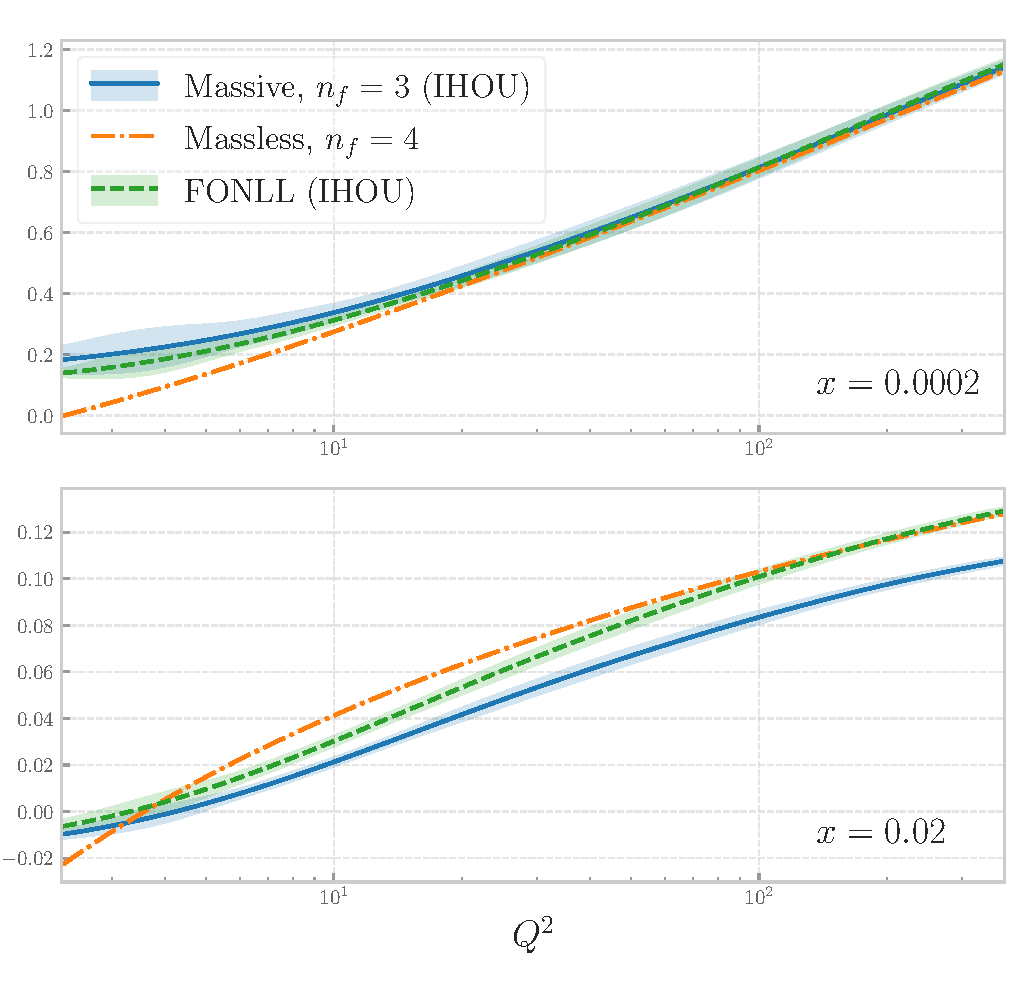
\includegraphics[width=0.89\textwidth]{figures/F2_charm_n3lo.pdf}
        \caption*{$F_2^{(c)}$}
      \end{figure}
    \end{column}
  \end{columns}

  % Up to NNLO, FONLL was implemented expressing the terms in the r.h.s in terms of $\alpha_s$ and PDFs defined in the massless scheme

  % FONLL is now implemented at ``observable level'' with simultaneous PDFs in different flavour number schemes, made possible thanks to the new \texttt{EKO} evolution code and \texttt{yadism} DIS library


\end{frame}


\begin{frame}{DIS structure functions}
  \begin{figure}[!t]
    \centering
    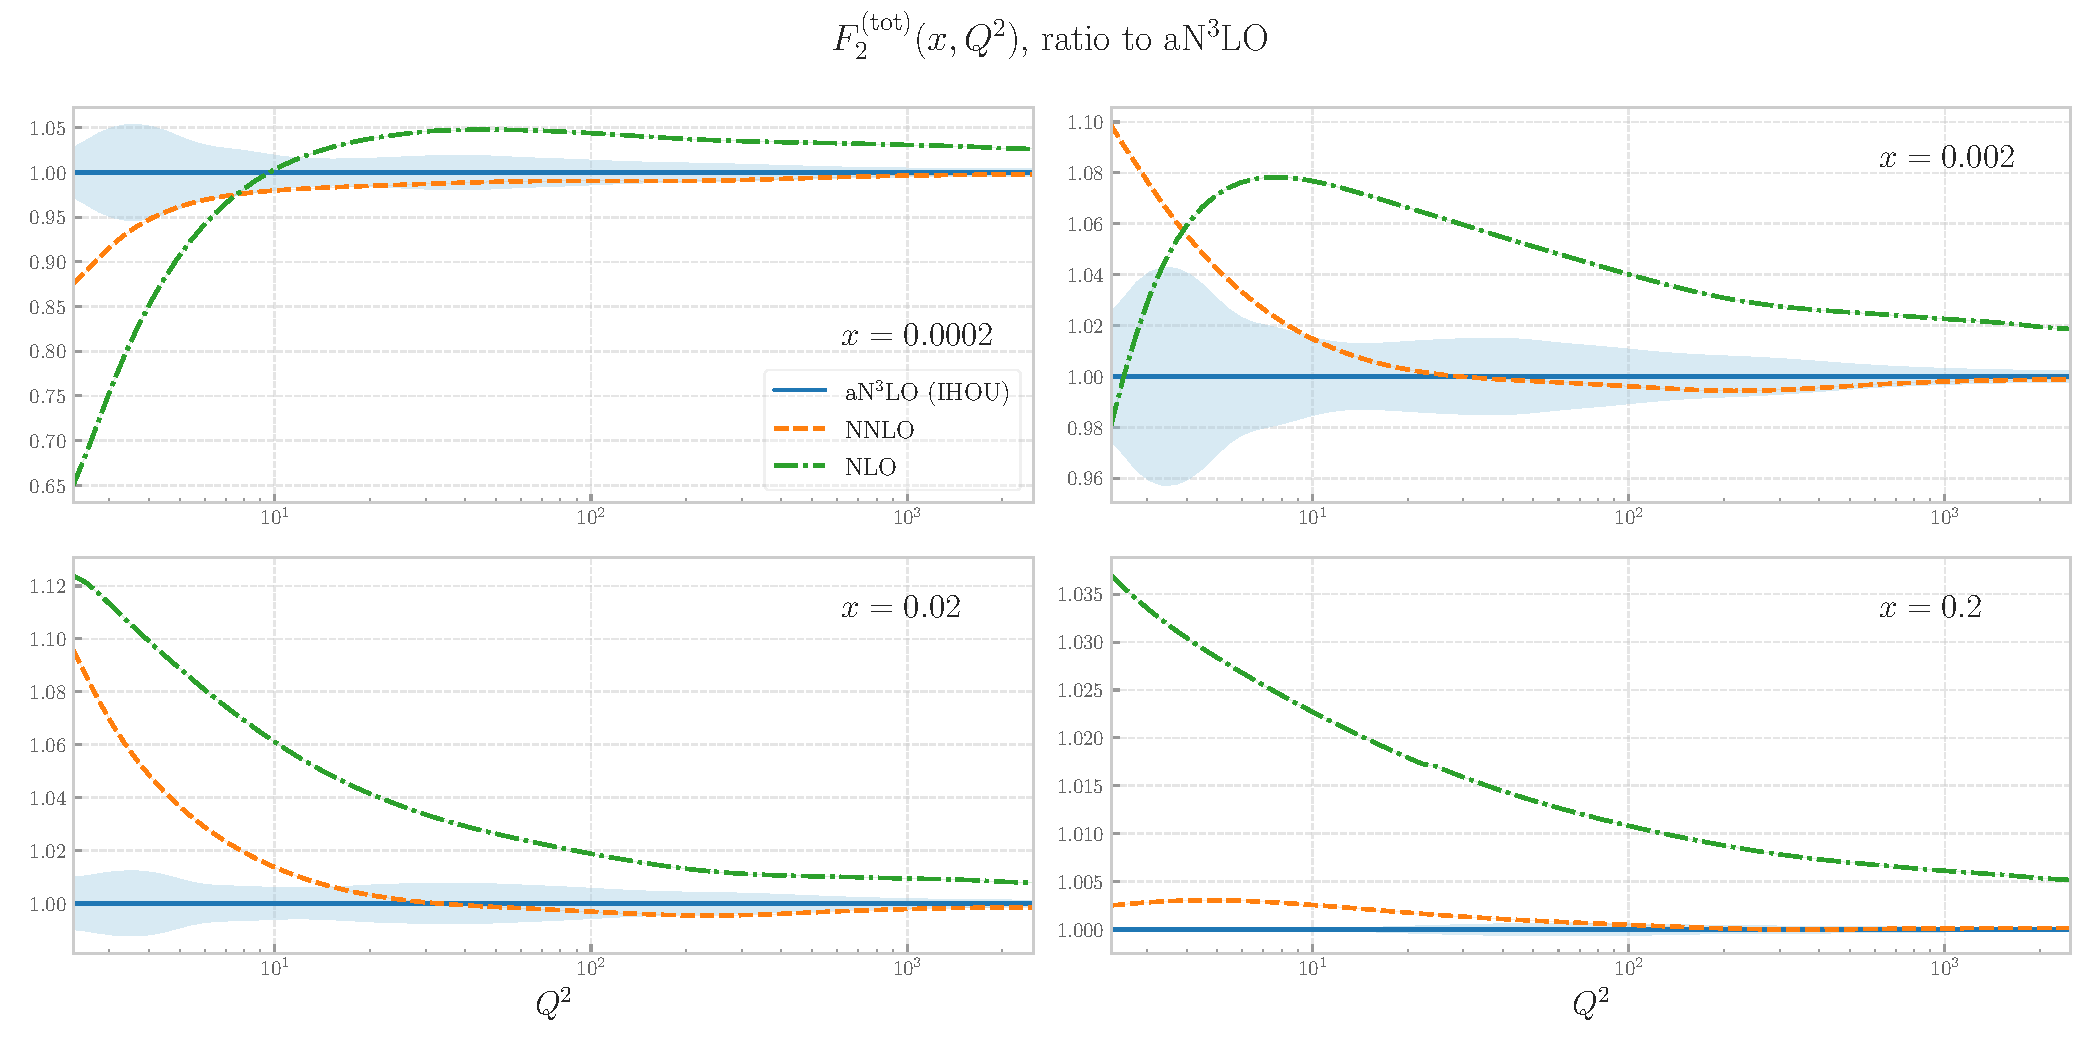
\includegraphics[width=0.75\textwidth]{figures/F2_total.pdf}
  \end{figure}
  \begin{itemize}
    \item The uncertainty band corresponds to IHOU of the massive coefficient functions
    \item N3LO corrections are significant at low-$Q$
  \end{itemize}
\end{frame}


\begin{frame}{Perturbative convergence}
  \begin{figure}[!t]
    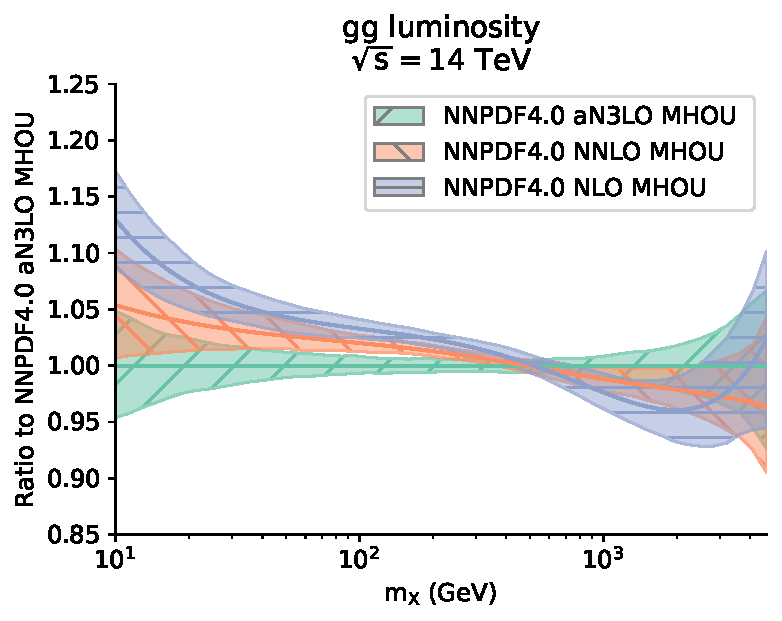
\includegraphics[width=.4\textwidth]{figures/gg_plot_lumi1d_convergence.pdf}
    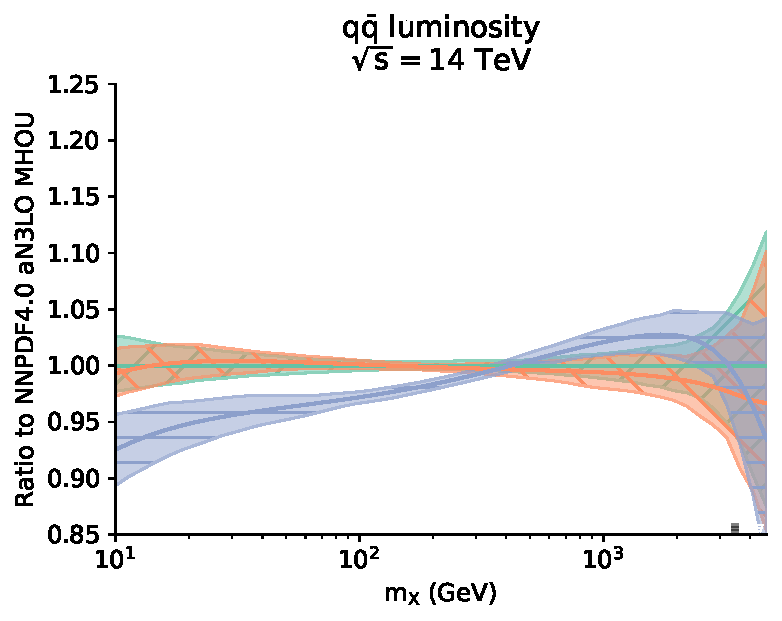
\includegraphics[width=.4\textwidth]{figures/qqbar_plot_lumi1d_convergence.pdf}
  \end{figure}
  \begin{itemize}
    \item Moderate impact of N3LO corrections, especially for the quark luminosities
    \item $\sim2\%$ suppression of $gg$ luminosity around the Higgs mass
  \end{itemize}
\end{frame}

\begin{frame}{Impact of MHOUs at N3LO}
  \begin{figure}[!t]
    \centering
    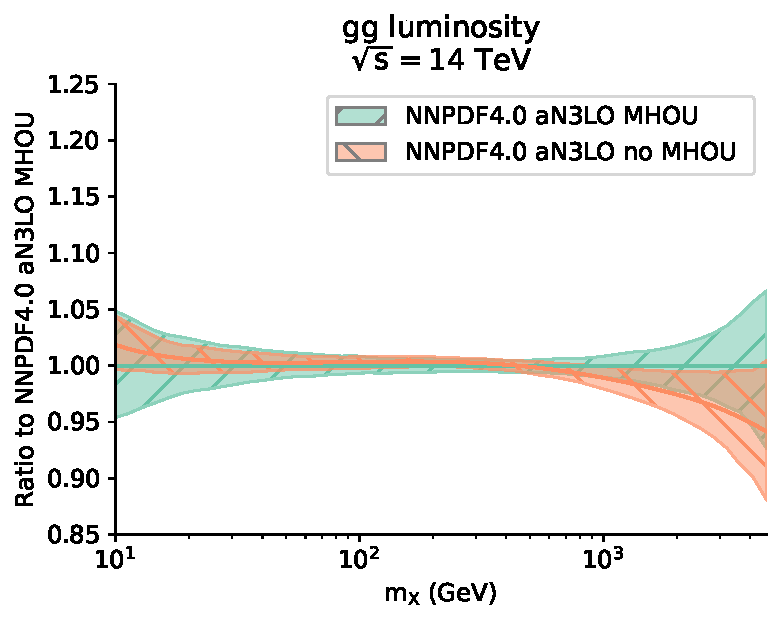
\includegraphics[width=0.45\textwidth]{figures/gg_plot_lumi1d.pdf}
    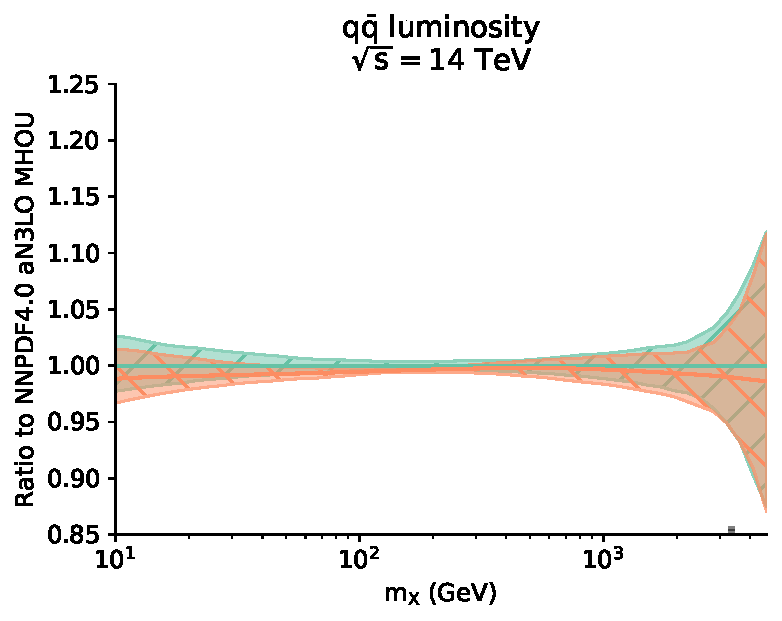
\includegraphics[width=0.45\textwidth]{figures/qqbar_plot_lumi1d.pdf}
  \end{figure}
  \begin{itemize}
    \item Non-negligible impact of MHOUs even at N3LO
    \item[$\Rightarrow$] reason to include exact N3LO calculations for hadronic processes
  \end{itemize}
\end{frame}


\begin{frame}{Incomplete higher order uncertainties covmat}
  \begin{itemize}
    \item We construct an IHOU matrix following a similar approach by varying the subleading functions
    \item IHOU are independent of MHOU so the uncertainties are added in quadrature
    $$C = C_\mathrm{exp}+C_\mathrm{MHOU}+C_\mathrm{IHOU}$$
  \end{itemize}

  \begin{columns}
    \begin{column}{0.49\textwidth}
      \begin{figure}[!t]
        \centering
        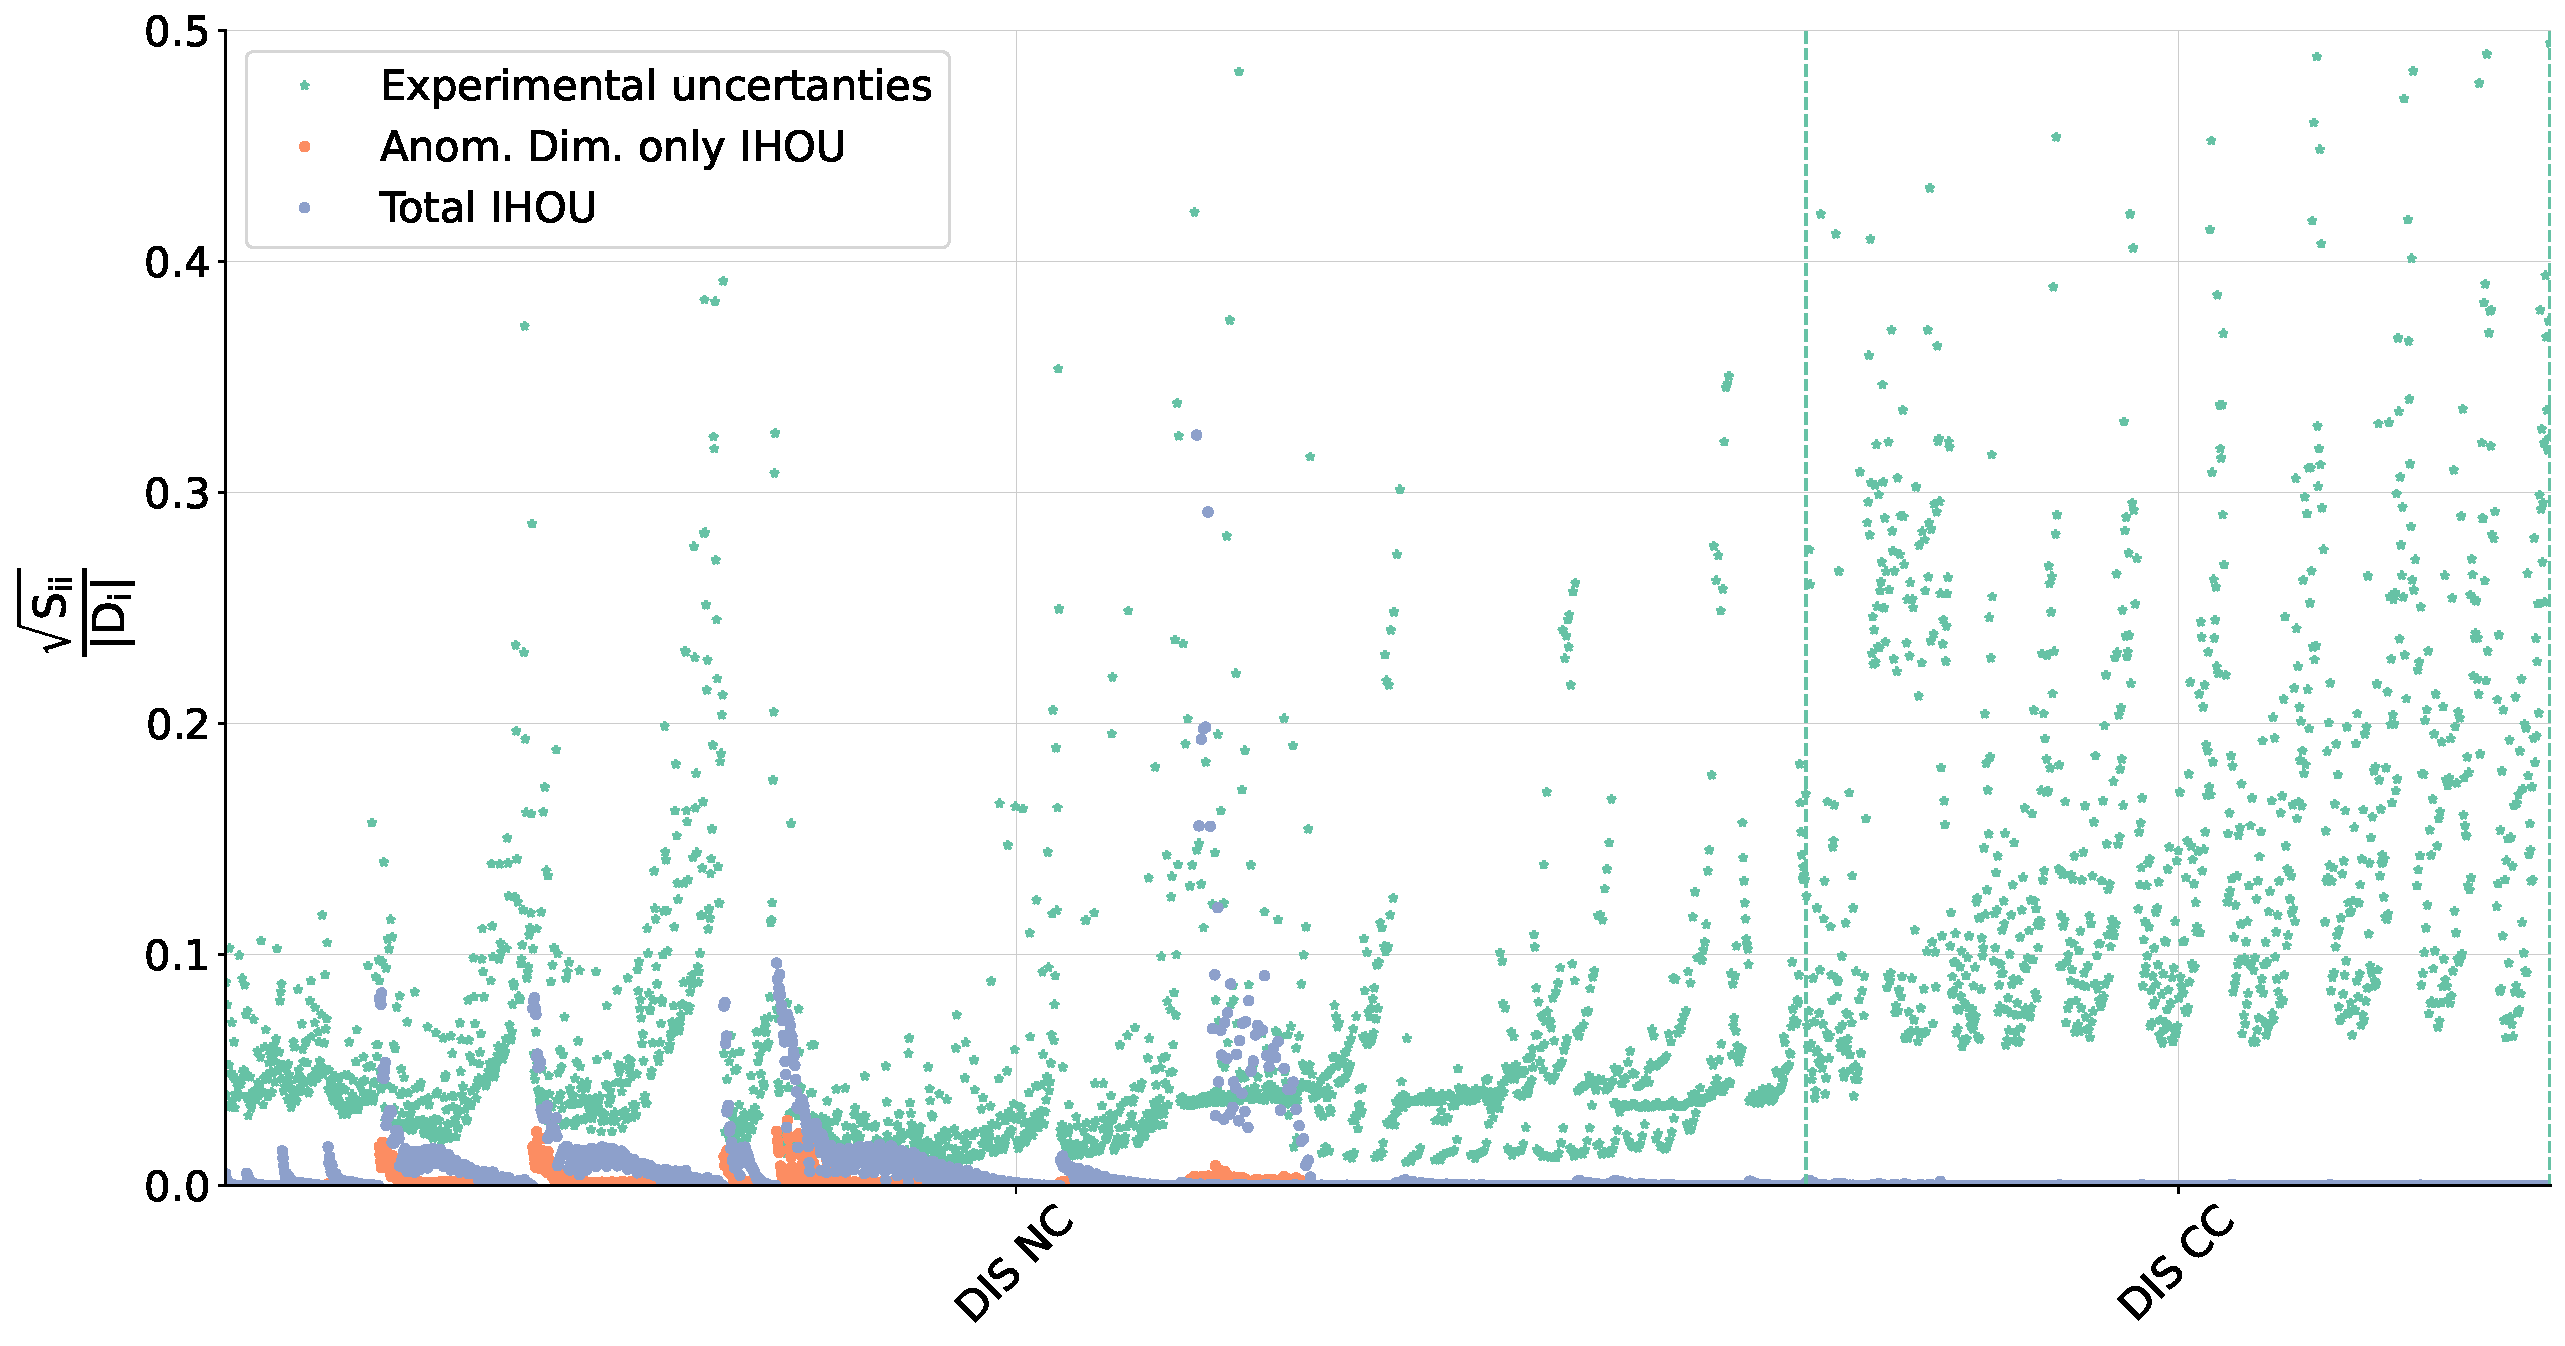
\includegraphics[width=.9\textwidth]{figures/diag_cov_dis_ihou.pdf}
        \caption*{IHOU have a large effect on small-$x$, low-$Q$ DIS data
        }
      \end{figure}
    \end{column}
    \begin{column}{0.49\textwidth}
      \begin{figure}[!t]
        \centering
        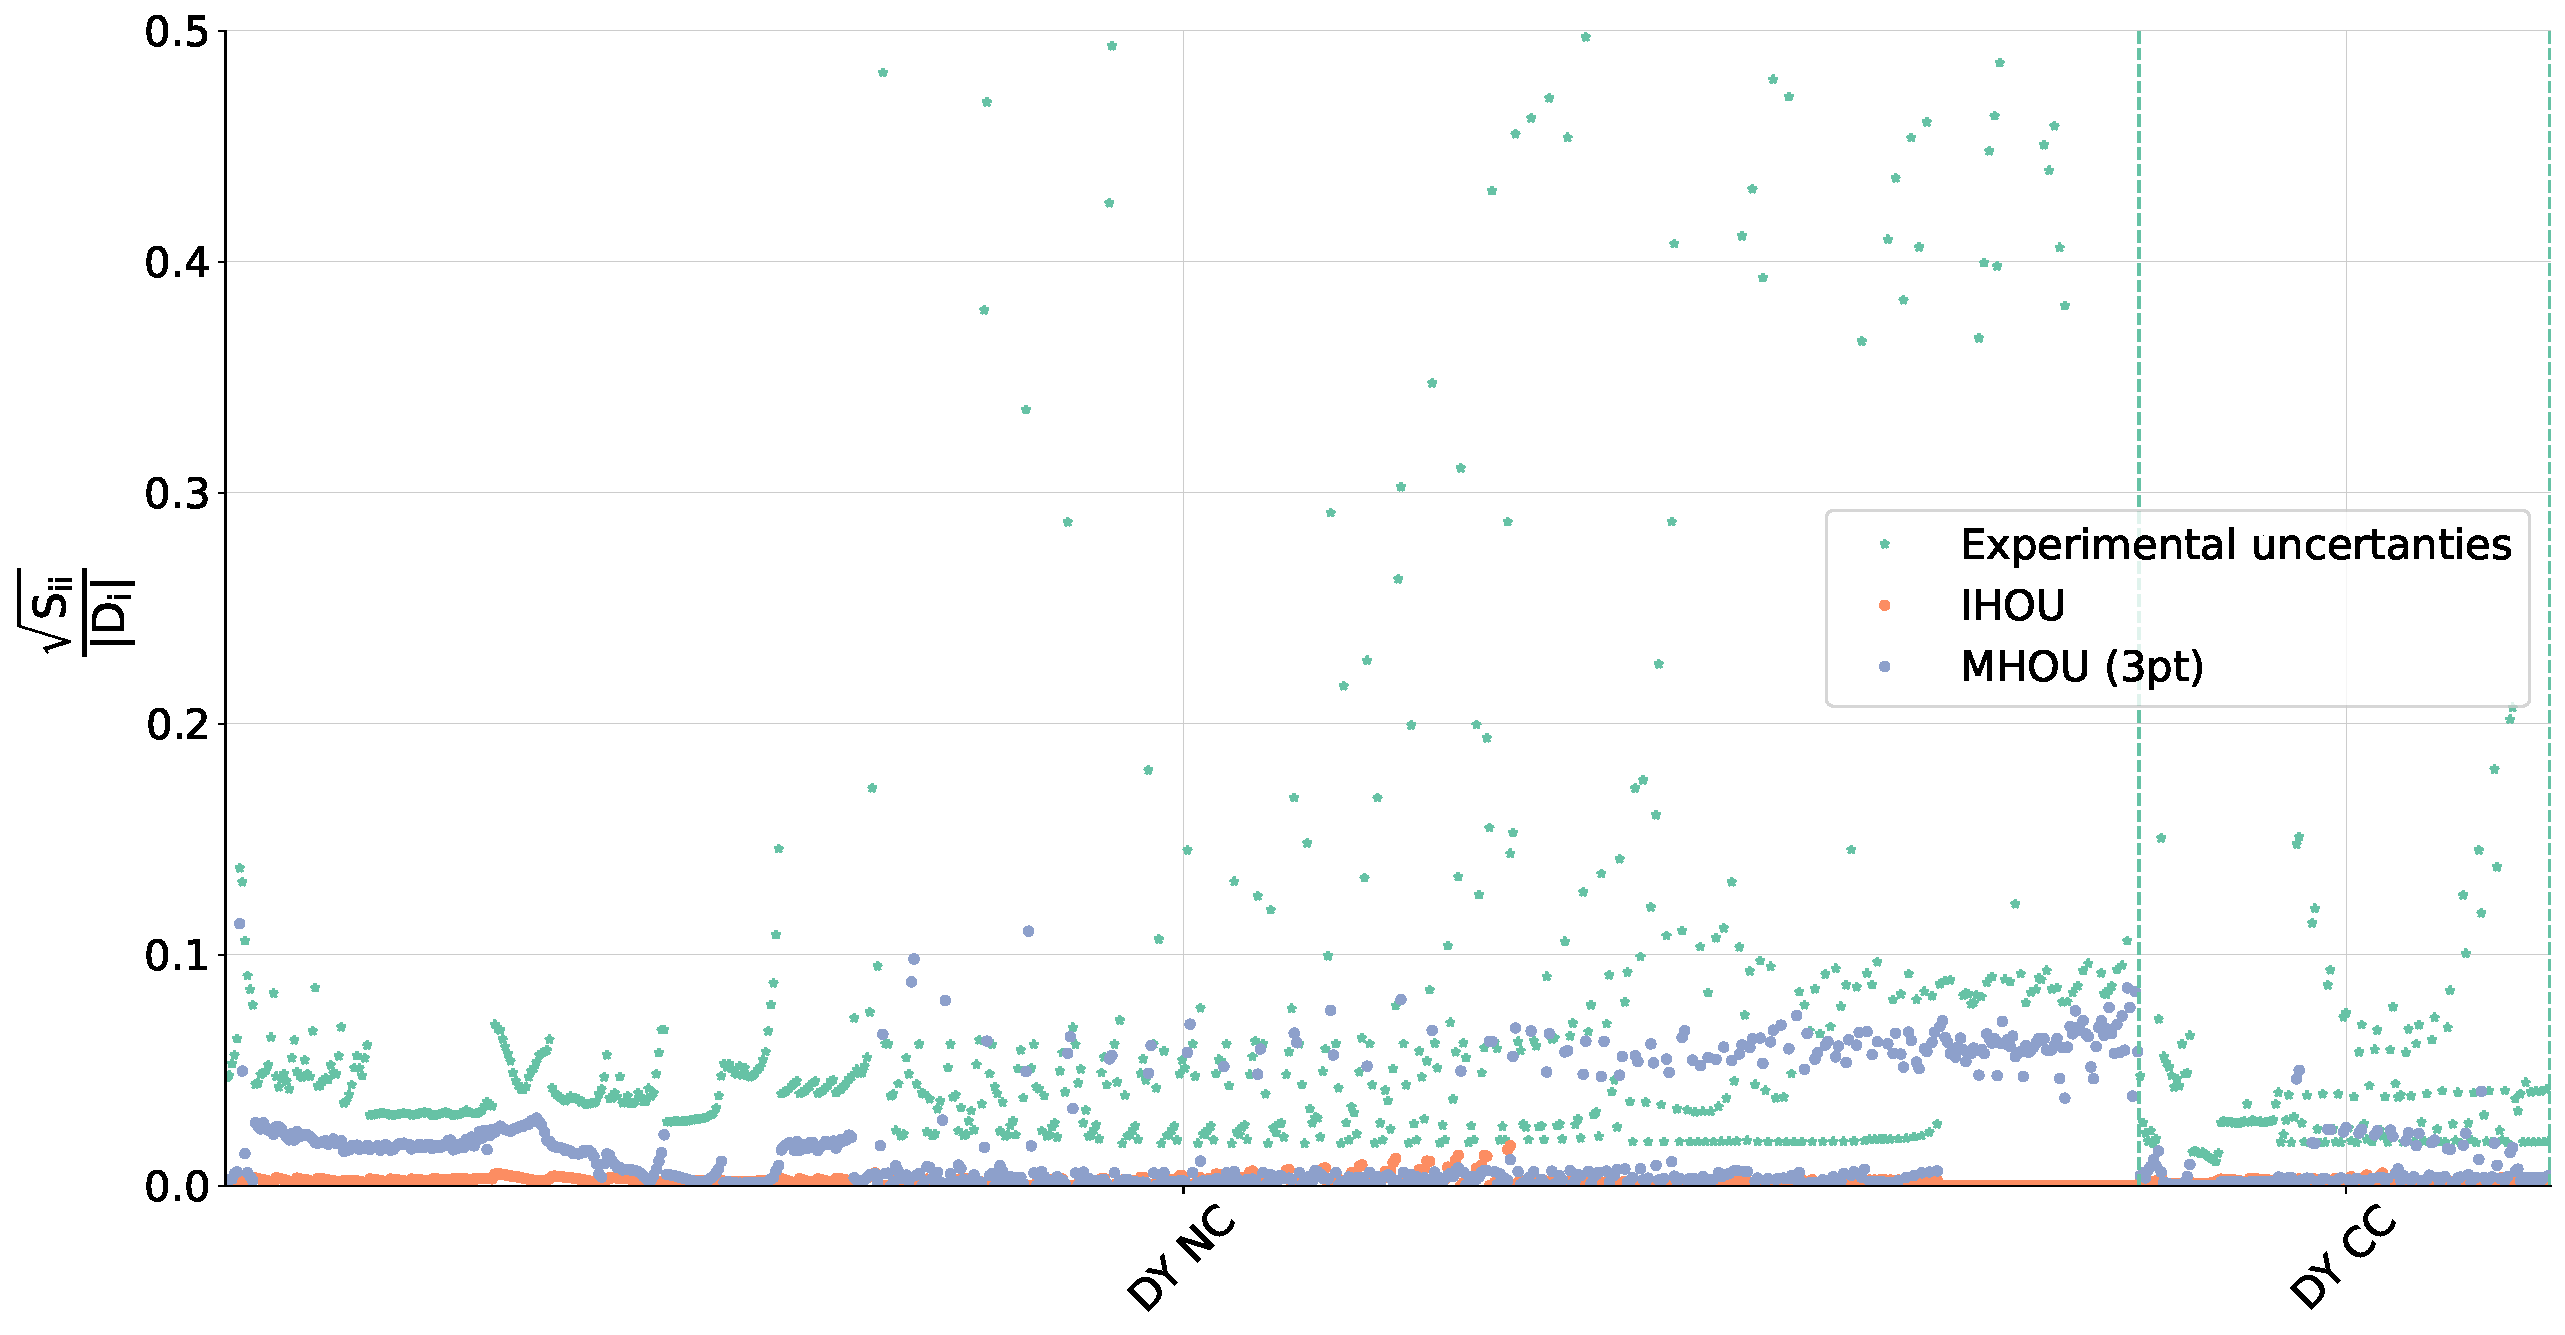
\includegraphics[width=.9\textwidth]{figures/diag_cov_dy_ihou_3pt_mhou.pdf}
        \caption*{NNLO MHOU included where N3LO not available \\
          MHOU can similar magnitude as the experimental uncertainty
        }
      \end{figure}
    \end{column}
  \end{columns}


\end{frame}



\begin{frame}{Determination of the photon PDF}
  \begin{columns}[T]
    \begin{column}{0.59\textwidth}
      Initially the photon PDF has been determined in different ways:
      \begin{itemize}
        \item physical model: sensitive to underlying model
        \item fitting: data does not provide strong constraints
      \end{itemize}

      \vspace*{0.5em}
      However with the LUXqed approach it can be computed perturbatively \\
      based on the observation that the heavy-lepton production cross-section can be written in two ways:
      \begin{itemize}
        \item in terms of structure functions $F_2$, $F_L$
        \item in terms of PDFs (including the photon)
      \end{itemize}

      \vspace*{0.5em}
      luxQED result {\color{gray}\small[Manohar, Nason, Salam, Zanderighi: 1607.04266, 1708.01256]}:
      \vspace*{-0.8em}
      \begin{equation*}
        \begin{split}
          & x \gamma(x, \mu^2)
          =
          \frac{2}{\alpha (\mu^2)} \int\limits_x^1 \frac{dz}{z}
          \Biggl\{ \int_{m_p^2x^2 \over 1-z}^{\mu^2 \over 1-z} \frac{dQ^2}{Q^2}
          \alpha^2(Q^2) \Biggl[ -z^2 F_L(x/z, Q^2) \\
          & + \left( z P_{\gamma q}(z) + \frac{2 x^2 m_p^2}{Q^2} \right)
          F_2(x/z, Q^2)\Biggr] - \alpha^2(\mu^2) z^2 F_2(x/z, \mu^2)\Biggr\}
        \end{split}
      \end{equation*}
    \end{column}

    \begin{column}{0.39\textwidth}
      \vspace*{-2.5em}
      \begin{figure}
        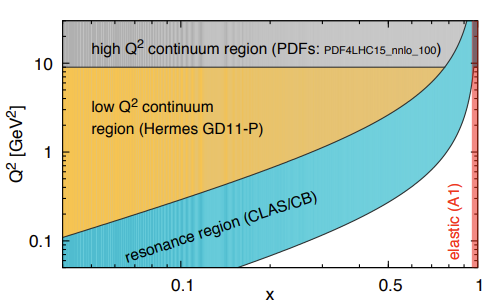
\includegraphics[width=0.89\textwidth]{figures/dataluxqed.png}
        \caption*{Input to construct $F_2$ and $F_L$}
        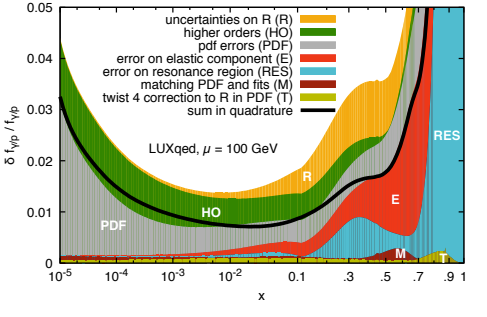
\includegraphics[width=0.89\textwidth]{figures/luxQED_uncs.png}
        \caption*{Sources of uncertainty}
      \end{figure}
    \end{column}
  \end{columns}
\end{frame}


\begin{frame}{LUXqed PDF determinations}
  LUXqed has been used in all of the most recent QED PDFs:
  \begin{itemize}
      \item LUXqed\_plus\_PDF4LHC15 {\color{gray}\small [1607.04266]}
      \item LUXqed17\_plus\_PDF4LHC15 {\color{gray}\small [1708.01256]}
      \item MMHT2015qed {\color{gray}\small [1907.02750]}
      \item NNPDF3.1luxQED {\color{gray}\small [1712.07053]}
      \item CT18lux and CT18qed {\color{gray}\small [2106.10299]}
      \item MSHT20QED {\color{gray}\small [2111.05357]}
      \item MSHT20qed\_an3lo {\color{gray}\small [2312.07665]}
      \item NNPDF4.0QED {\color{gray}\small [2401.08749 ]}
  \end{itemize}
\end{frame}


\begin{frame}[t]{Data in NNPDF4.0}
  \begin{center}
    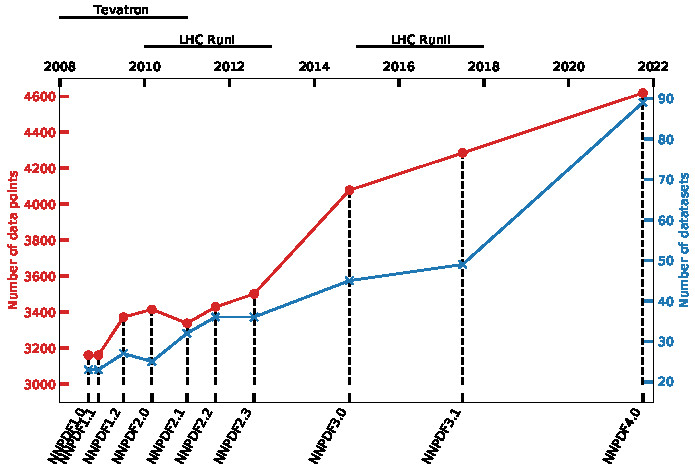
\includegraphics[width=0.7\textwidth]{NNPDF_data_history.pdf}
  \end{center}
  Better data $\rightarrow$ higher precision and accuracy
\end{frame}


\begin{frame}{Data in NNPDF4.0}
  \begin{columns}
      \column{0.7\linewidth}
          \begin{figure}
              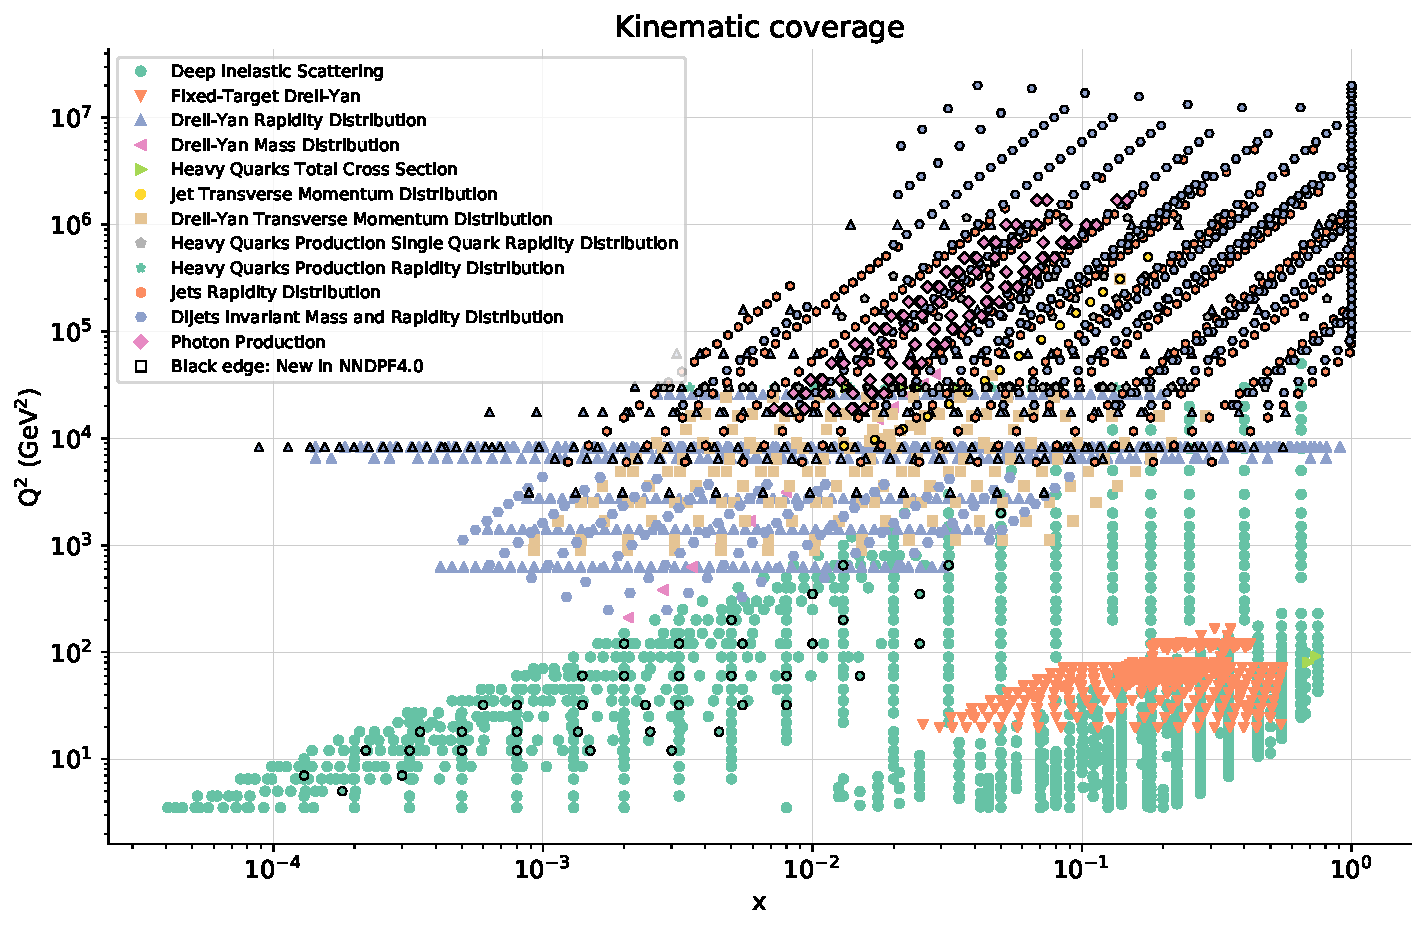
\includegraphics[width=0.9\textwidth]{Markers0_plot_xq2}
          \end{figure}
      \column{0.3\linewidth}

          \vspace*{2em}
          More than 4000 datapoints\\
          and 13 processes!\\
          \vspace*{1em}
          New processes:
          \begin{itemize}
              \item direct photon
              \item single top
              \item dijets
              \item W+jet
              \item DIS jet
          \end{itemize}
  \end{columns}
\end{frame}

\begin{frame}{Validating the methodology}
  We thus have two possible methodologies to determine $\alpha_s$, but how can we trust they give the correct answer?

  \vspace*{1em}
  \begin{columns}

    \begin{column}{0.49\textwidth}
      Basic idea is that of a closure test:
      \begin{enumerate}
        \item generate data with theory predictions $T_0$ for a given value of $\alpha_s$, e.g. $0.118$ -- centre of the diagram

        \item sample the covariance matrix to simulate experimental sampling $\eta$ \\
        $\color{green}y_0 = T_0 + \eta$, \quad $\eta  \overset{\text{i.i.d.}}{\sim} \mathcal{N}(0,\mathrm{Cov})$

        \item create many replicas by sampling on top of ${\color{green}}$ \\
        $y_\mathrm{rep} = {\color{green}} + \delta$, \quad $\delta  \overset{\text{i.i.d.}}{\sim} \mathcal{N}(0,\mathrm{Cov})$ -- the green circle

        \item perform fits to all replicas $y_\mathrm{rep}$ -- the blue circle

        \item repeat for many ${\color{green}}$

        \item[$\bullet$] usual \textbf{data-level closure test:} check if for 68\% of ${\color{green}}$ samples, $\color{blue}E_\epsilon$ is within 1$\sigma$ from $T0$

        \item \textbf{closure test of $\alpha_s$:} check if the same applies for the predictions of the $\alpha_s$ value.
      \end{enumerate}
    \end{column}
    \begin{column}{0.49\textwidth}
      \begin{figure}
        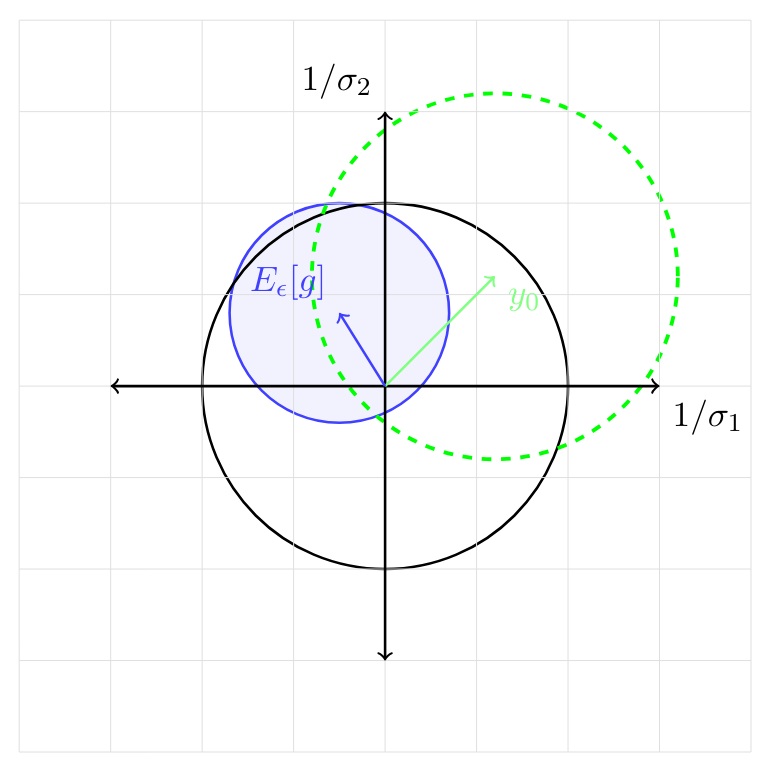
\includegraphics[width=0.99\textwidth]{geometric_closure_test.png}
        \caption*{\color{gray} \footnotesize Del Debbio, Giani, Wilson, \hyperlink{https://arxiv.org/abs/2111.05787}{2111.05787}}

      \end{figure}
    \end{column}
  \end{columns}

  \begin{center}
    \vspace*{1em}
    \only<2>{\textbf{Preliminary results based on 25 sampled $y_0$ suggests the ``correlated replicas'' method faithfully determines $\alpha_s$}}
  \end{center}
\end{frame}

\begin{frame}{Process sensitivity}
  \begin{itemize}
    \item Impact of PDF-$\alpha_s$ correlations can be up to a factor 2
    \item Estimate the pull from different processes by comparing $\alpha_s$ determinations from $\chi^2$ calculated to a subset of the data
    \item Global fits account for the effects of all data!
  \end{itemize}
  \begin{figure}
    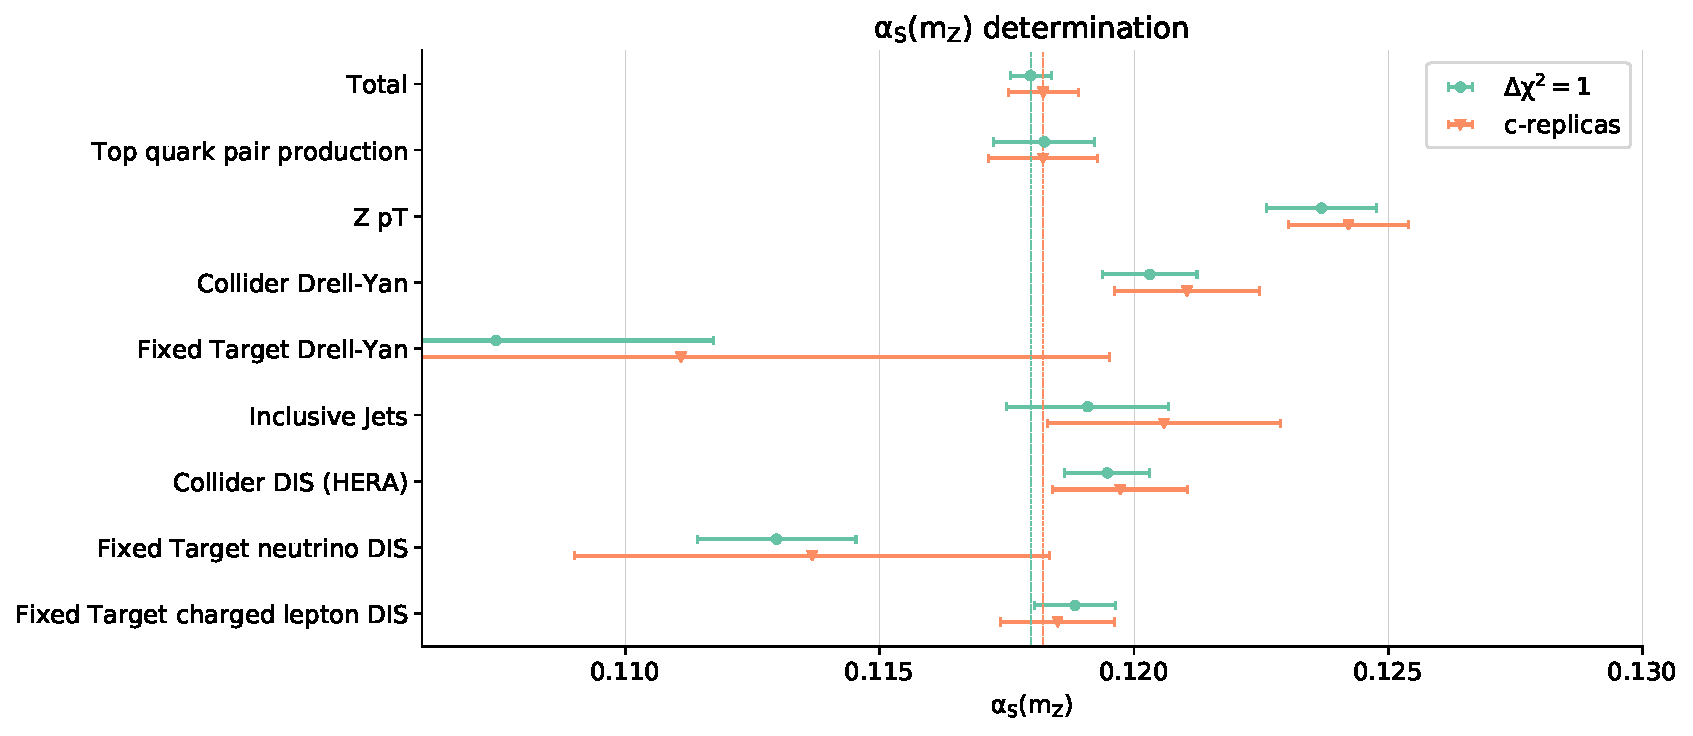
\includegraphics[width=0.7\textwidth]{as_determination_central_NNLO.pdf}
    \caption*{\color{gray} \footnotesize NNPDF, \hyperlink{https://arxiv.org/abs/1802.03398}{1802.03398}}
  \end{figure}
\end{frame}



\begin{frame}[t]{The NNPDF approach: an importance sampling}
  \begin{itemize}
    \item Importance sampling produces Gaussian posterior distribution
    \item All replicas equally likely
  \end{itemize}
  \begin{center}
    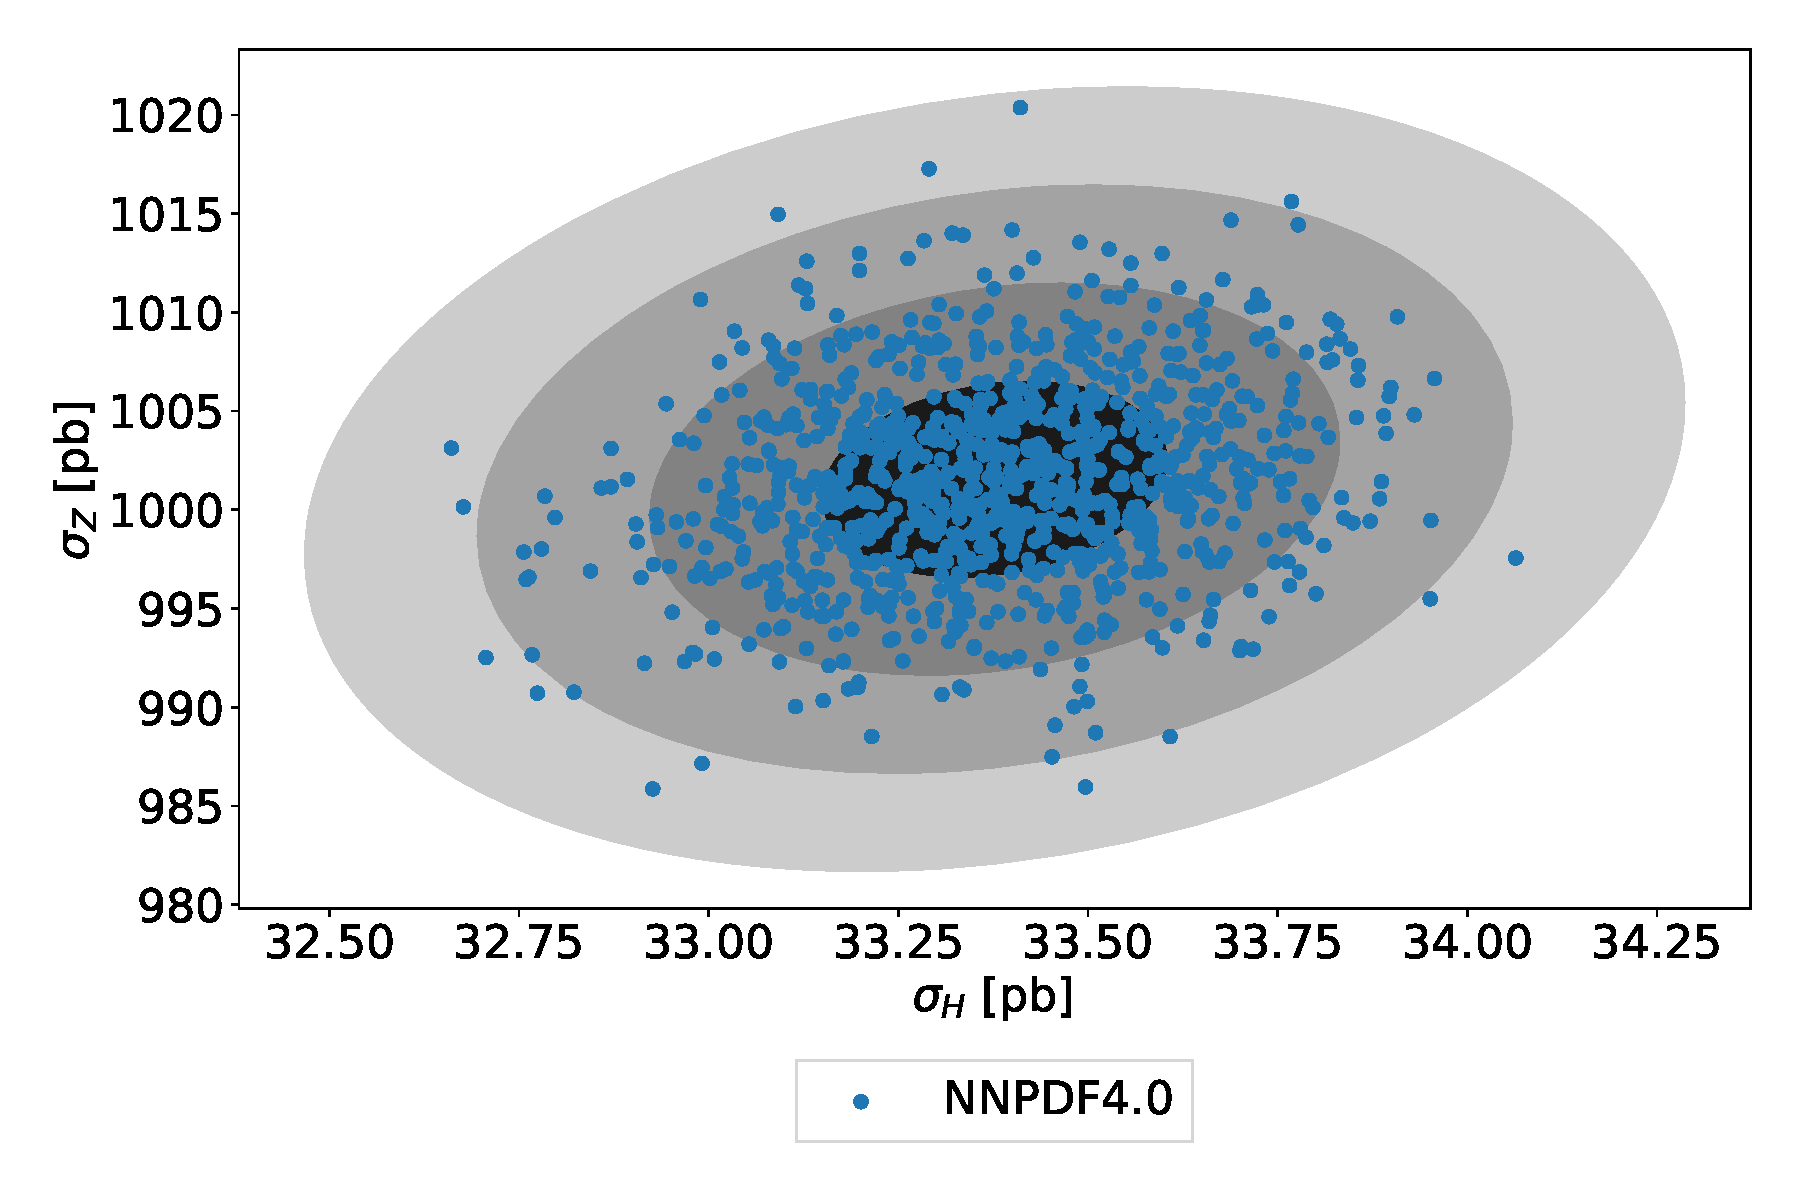
\includegraphics[width=0.5\textwidth]{nnpdf40_dist.pdf}
  \end{center}
\end{frame}



\begin{frame}[t]{Parametrization}
  \begin{columns}[T]
      \begin{column}{0.48\textwidth}
        Neural network: universal interpolator
        \vspace*{0.3cm}
        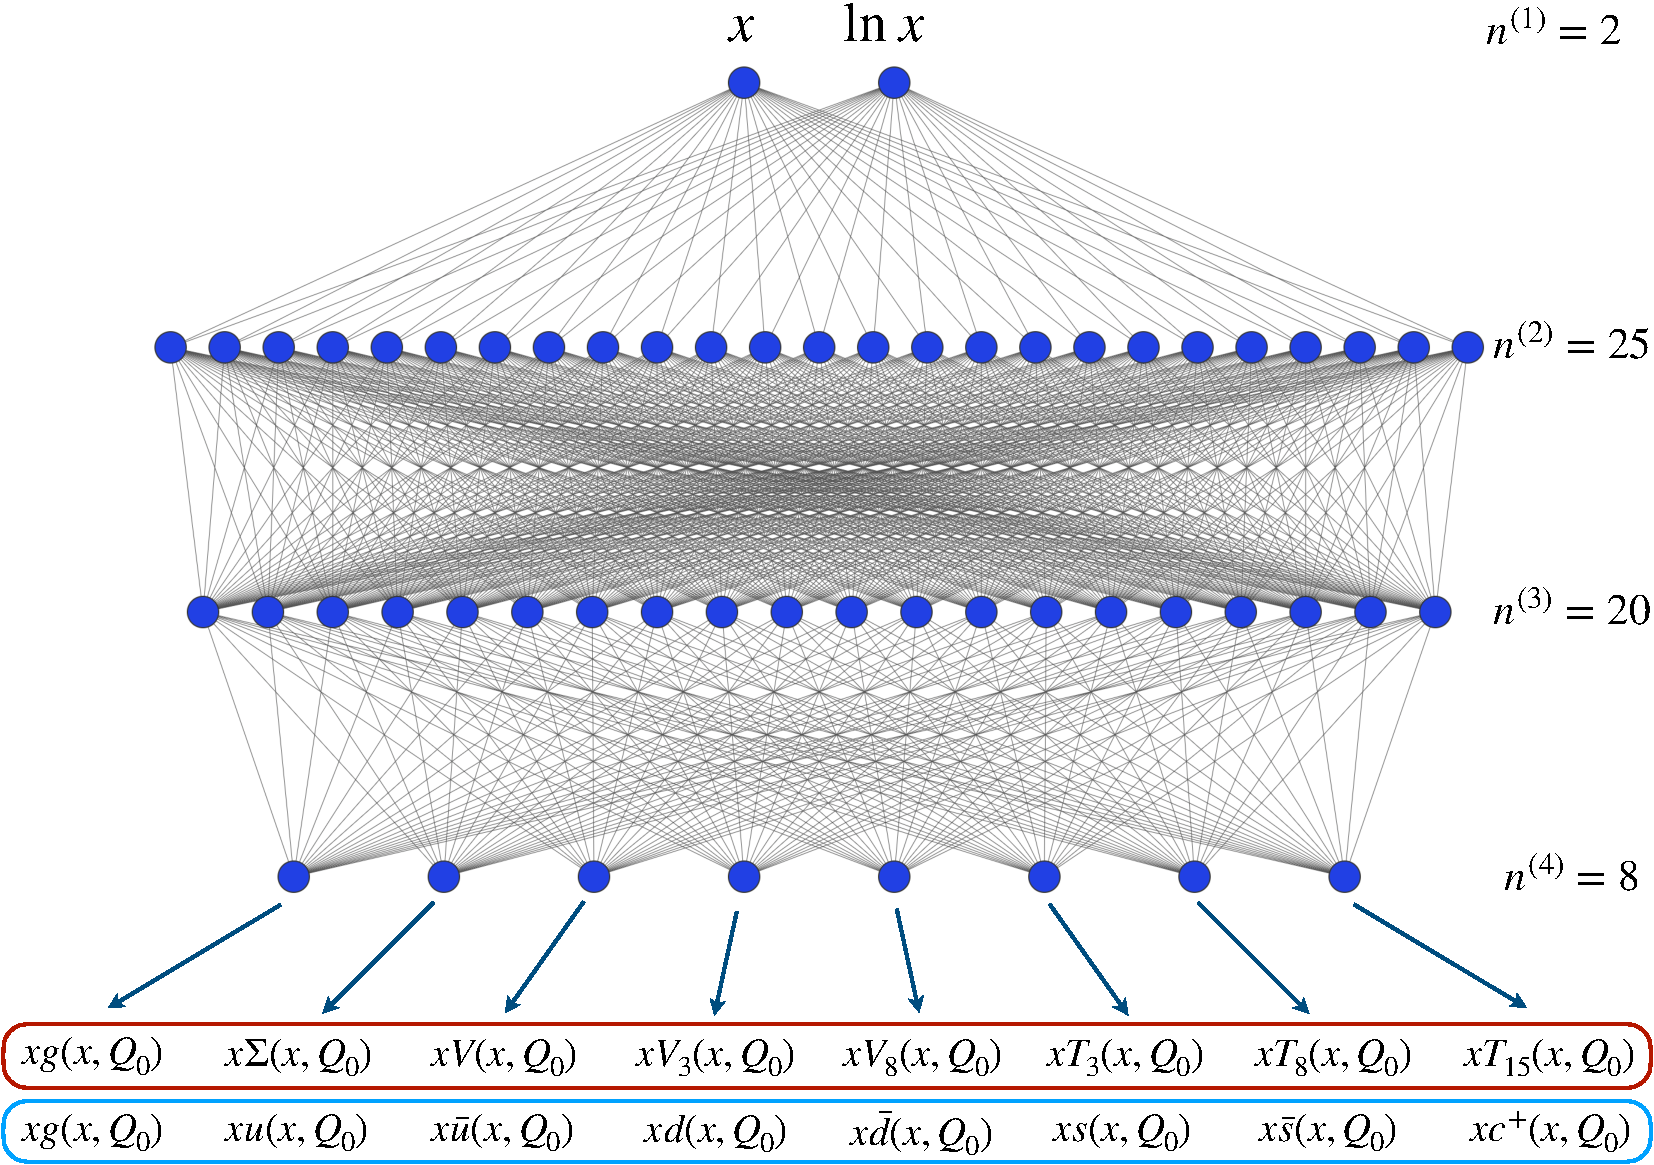
\includegraphics[width=1.0\textwidth]{NNarch}
        \begin{equation*}
            f_{i}\left(x, Q_{0}\right)=x^{-\alpha_{i}}(1-x)^{\beta_{i}} \mathrm{NN}_{i}(x)
        \end{equation*}
      \end{column}
      \begin{column}{0.48\textwidth}
        Physical constraints:
        \begin{itemize}
            \item PDF positivity [JHEP 11 (2020)]
            \item Integrability of nonsinglet distributions (Gottfried sum rules)
        \end{itemize}
        \vspace*{0.3cm}
        \begin{itemize}
          \item Train by minimizing $\chi^2$ loss function comparing data to prediction\\
        \end{itemize}
      \end{column}
  \end{columns}
\end{frame}


\usetikzlibrary{shapes, arrows}
\usetikzlibrary{decorations.pathreplacing}
\usetikzlibrary{positioning, calc}
\tikzstyle{fitted} = [rectangle, minimum width=5cm, minimum height=1cm, text centered, draw=black, fill=red!30]
\tikzstyle{operations} = [rectangle, rounded corners, minimum width=2cm,text centered, draw=black, fill=red!30]
\tikzstyle{roundtext} = [rectangle, rounded corners, minimum width=2cm, minimum height=0.8cm, text centered, draw=black, fill=red!30]
\tikzstyle{n3py} = [rectangle, rounded corners, minimum width=3cm, minimum height=1cm, text centered, draw=black, fill=green!30]
\tikzstyle{myarrow} = [thick,->,>=stealth]
\tikzstyle{line} =[draw, -latex']
\tikzstyle{decision} = [diamond, draw, fill=red!20, text width=7.5em, text centered,  inner sep=0pt, minimum height=2em, aspect=4]
\tikzstyle{cloud} = [draw, ellipse,fill=green!20, minimum height=2em]
\tikzstyle{inout} = [rectangle, draw, fill=green!20, text width=9.5em, text centered, rounded corners, minimum height=2em, minimum width=10em]
\tikzstyle{block}=[rectangle, draw, fill=blue!20, text width=9.5em,
                   text centered, rounded corners, minimum height=2em,
                   minimum width=10em]
\tikzstyle{arrow} = [thick,->,>=stealth]

\pgfdeclarelayer{bg}    % declare background layer
\pgfsetlayers{bg,main}  % set the order of the layers (main is the standard layer)

\begin{frame}[t]{Training the neural network}
  \begin{itemize}
    \item Optimize using a gradient descent algorithm
    \item NN should generalize the underlying law, but if trained to long noise is fitted
  \end{itemize}
  \begin{columns}[T]
    \begin{column}[T]{0.49\textwidth}
      Cross-validation
      \begin{itemize}
        \item Divide data into {\color{blue} training} and {\color{orange} validation}
        \item Minimize training $\chi^2$
        \item {\color{red} Stop} if {\color{orange} validation} $\chi^2$ no longer improves
      \end{itemize}
      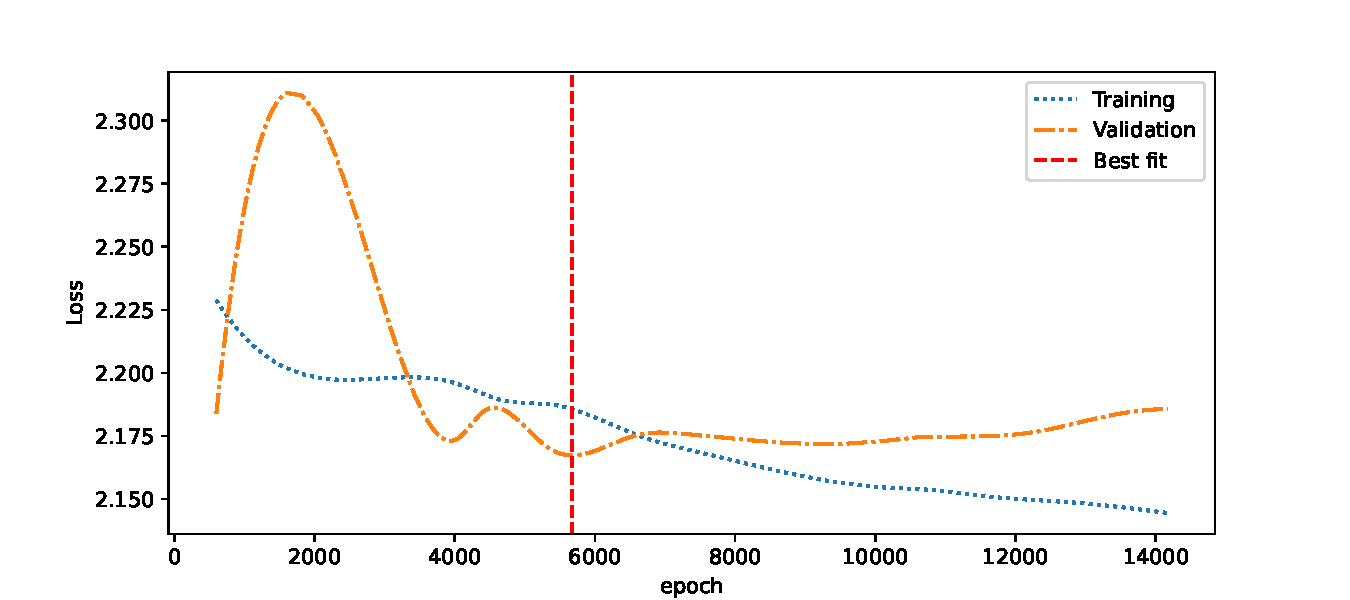
\includegraphics[width=0.9\textwidth]{trvl.pdf}
    \end{column}
    \begin{column}{0.49\textwidth}
      \begin{figure}
        \centering
        \resizebox{\columnwidth}{!}{
        \begin{tikzpicture}[node distance = 1.5cm, scale=0.1]\small
            \definecolor{vp1}{RGB}{102,194,165}
            \definecolor{vp2}{RGB}{252,141,98}
            % Middle column
            \node (init) [roundtext, fill=vp1!30, minimum width=5.2cm] {next training step};
            \node (ccheck) [roundtext, fill=vp2!30, minimum width=4cm, minimum height=0.8cm, below of = init] {counter
                $>$ max};
            \node (pcheck) [roundtext, fill=vp2!30, minimum width=4cm, minimum height=0.8cm, below of = ccheck]
                {positivity fulfilled?};
            \node (xcheck) [roundtext, fill=vp2!30, minimum width=4cm, minimum height=0.8cm, below of = pcheck]
                {$\chi^2_\text{val}$ $<$ best $\chi^2$};
            \node (reset) [roundtext, fill=vp1!30, minimum width=5.2cm, below of = xcheck] {reset counter $\rightarrow$  best
                $\chi^2 = \chi^2_\text{val}$};Q

            % Off-center nodes
            \node (cplus) [roundtext, fill=vp2!30, left = 0.9cm of ccheck]
                {\ttfamily counter ++};
            \node (end) [roundtext, fill=vp2!30, right = 0.9cm of ccheck]
                {\ttfamily END};

            % Coordinates
            \coordinate[above of = cplus] (li);
            \coordinate[below of = cplus] (lp);
            \coordinate[below of = lp] (lx);
            \coordinate[below of = lx] (lr);


            % Arrows center
            \draw[myarrow] (init) -- (ccheck);
            \draw[myarrow] (ccheck) -- node[right] {No} (pcheck);
            \draw[myarrow] (pcheck) -- node[right] {Yes}(xcheck);
            \draw[myarrow] (xcheck) -- node[right] {Yes}(reset);

            % Arrows off-center
            \draw[myarrow] (ccheck) --  node[above] {Yes} (end);

            \draw[myarrow] (reset) -- (lr) -- (lx);
            \draw[myarrow] (xcheck) -- node[above] {No} (lx) -- (lp);
            \draw[myarrow] (pcheck) --  node[above] {No} (lp) -- (cplus);
            \draw[myarrow] (cplus) -- (li) -- (init);
        \end{tikzpicture}
        }
      \end{figure}
    \end{column}
  \end{columns}
\end{frame}


\begin{frame}[t]{Verify the importance sampling assumption}
  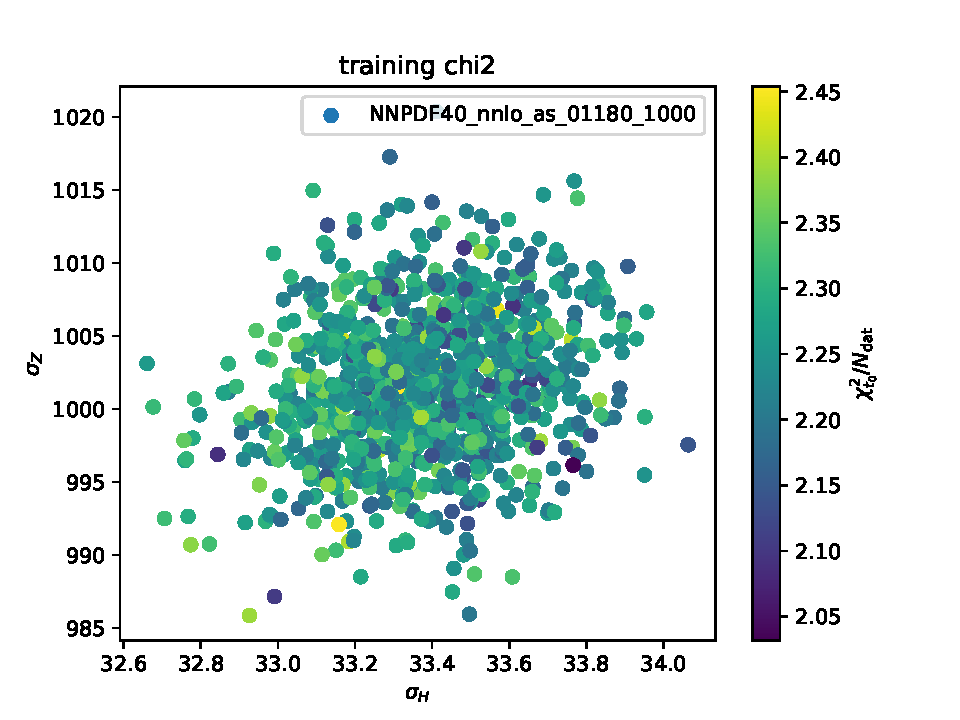
\includegraphics[width=0.49\textwidth]{chi2_training_chi2.pdf}
  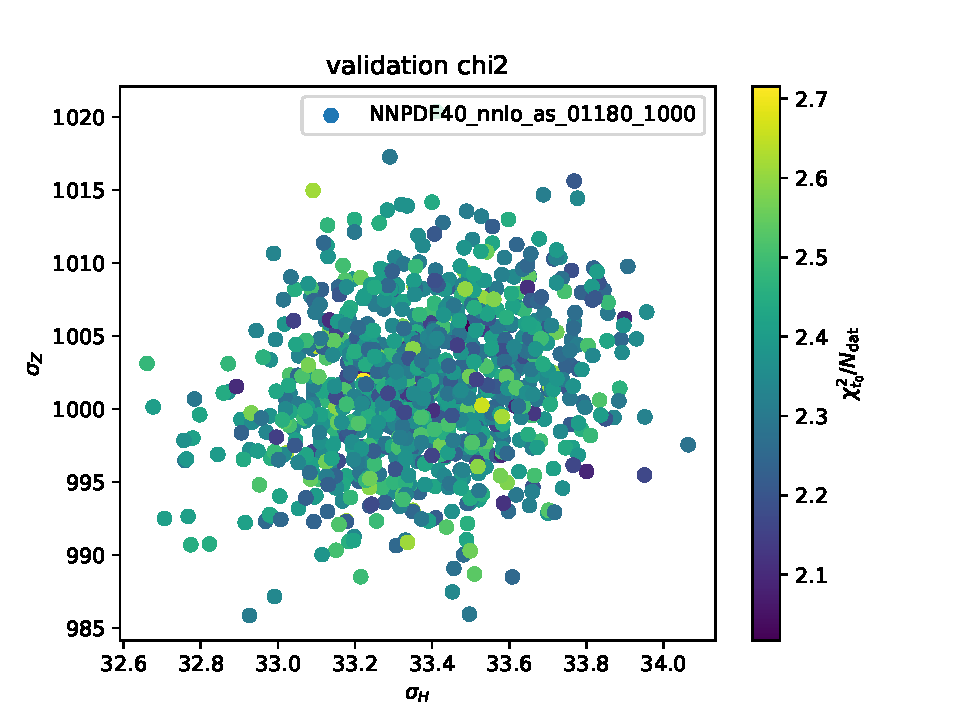
\includegraphics[width=0.49\textwidth]{chi2_validation_chi2.pdf}
  \begin{itemize}
    \item All PDF replicas are fitted equally well to their data replica
    \item Thus outliers correspond to unlikely data replicas
  \end{itemize}
\end{frame}

\begin{frame}[t]{Automated model selection}
  NNPDF aims to minimize sources of bias in the PDF:
  \begin{itemize}
      \item Functional form $\rightarrow$ Neural Network
      \item Model parameters $\rightarrow$ \textbf{Hyperoptimization}
  \end{itemize}
    \begin{columns}
        \begin{column}{0.48\textwidth}
            Scan over thousands of hyperparameter combinations and select the best one \\
            \vspace*{0.8em}
            {\bf k-fold cross-validation}: used to define the reward function based on a {\bf test dataset}\\
            \vspace*{0.8em}
            Objective function: \\
            $L=\textrm{mean}(\chi_1^2,\chi_3^2,\chi_2^2,\ldots, \chi_k^2)$

            \vspace*{0.3cm}
            Final step requires human input
        \end{column}
        \begin{column}{0.48\textwidth}
            \begin{center}
                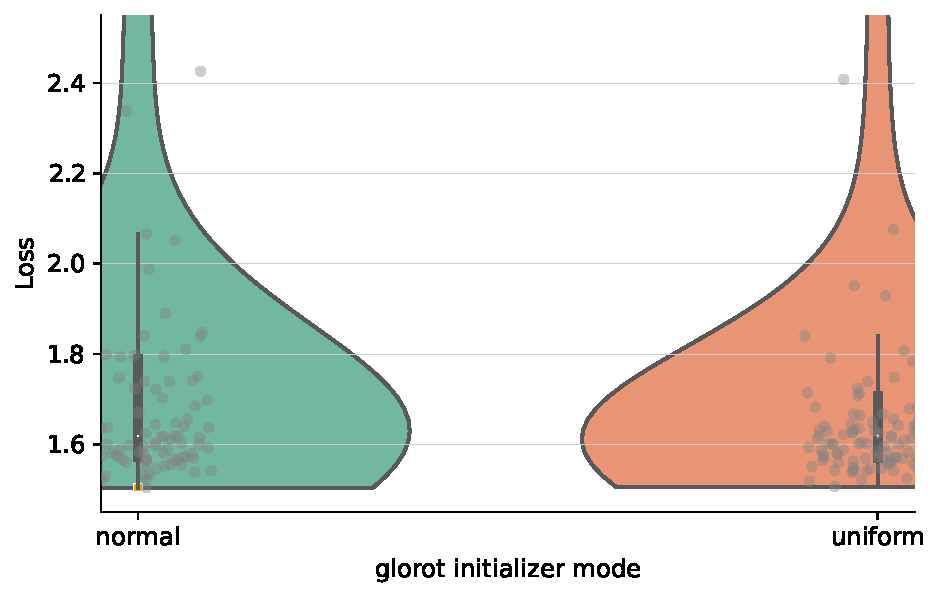
\includegraphics[width=0.48\textwidth]{sec_methodology_hyperopt_plot_initializer.pdf}
                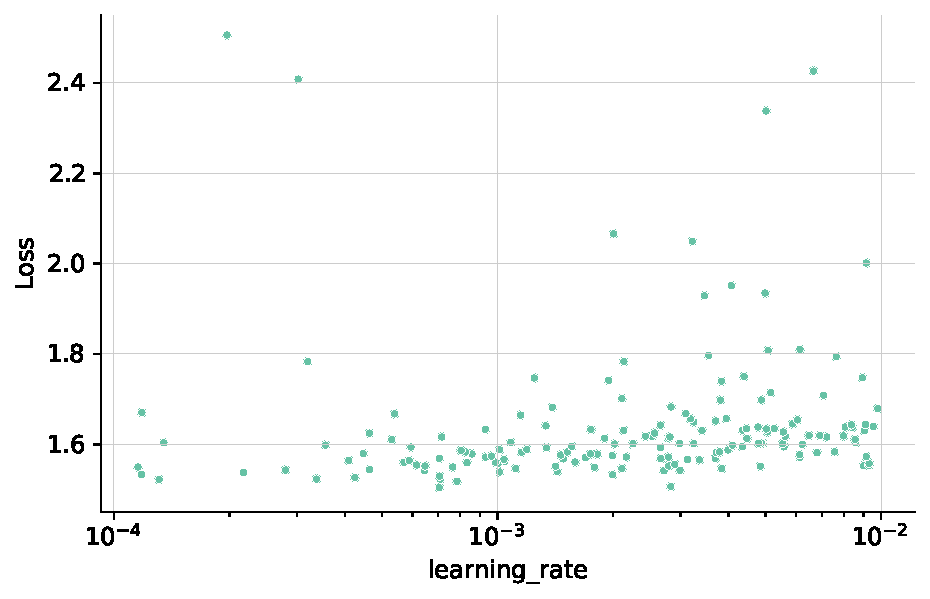
\includegraphics[width=0.48\textwidth]{sec_methodology_hyperopt_plot_lr.pdf} \\
                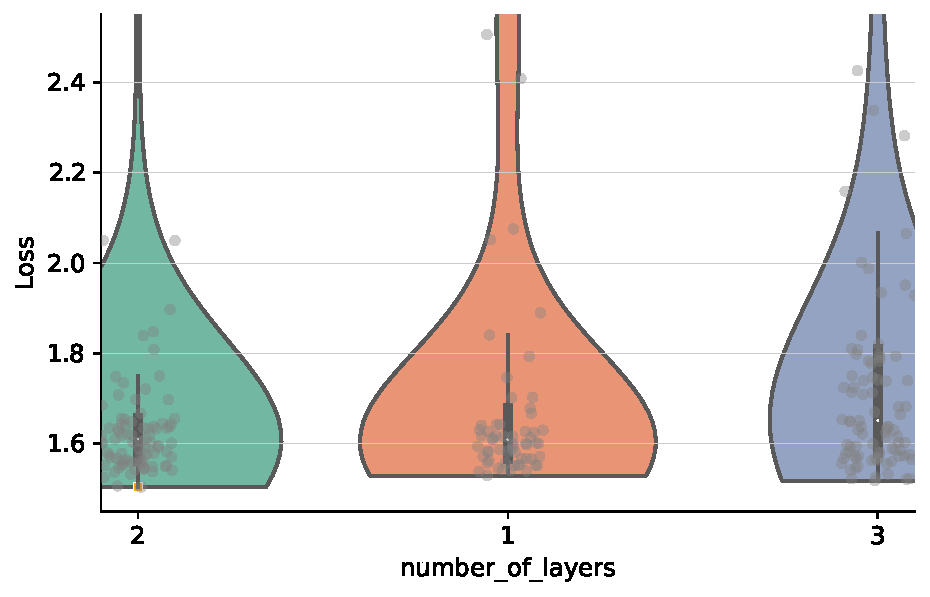
\includegraphics[width=0.48\textwidth]{sec_methodology_hyperopt_plot_number_of_layers.pdf}
                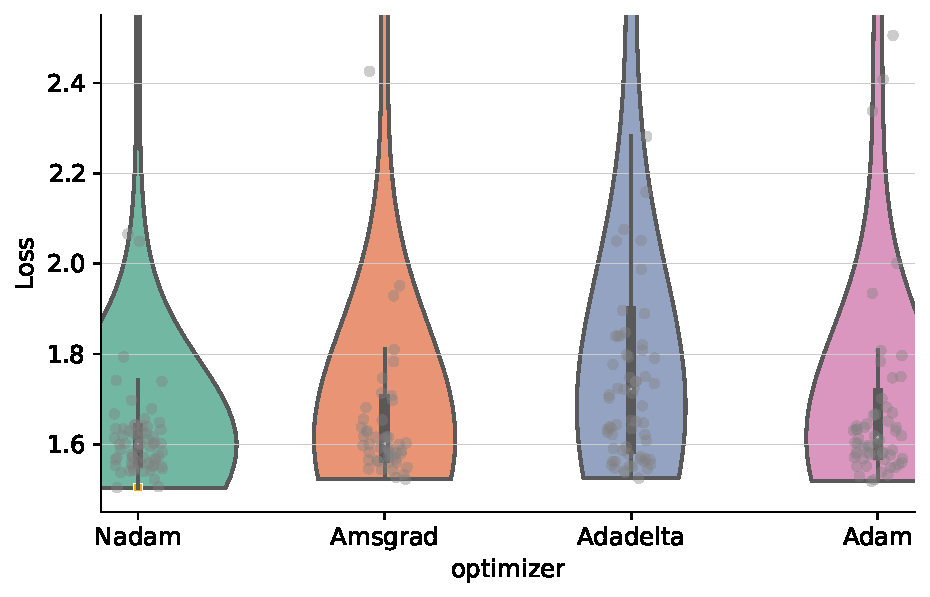
\includegraphics[width=0.48\textwidth]{sec_methodology_hyperopt_plot_optimizers.pdf}
            \end{center}
        \end{column}
    \end{columns}
\end{frame}


